\documentclass[iop,apj,twocolumn,twocolappendix,numberedappendix]{emulateapj}
\usepackage{apjfonts}
\usepackage{multirow}
\usepackage{textcomp}
\usepackage{amsmath}
\usepackage{microtype}
\usepackage{subfigure}
\usepackage{xcolor,ulem}
\usepackage[breaklinks=true]{hyperref}

%@arxiver{mass_boxes,Fig_mass_SNR,spin_cred_regions}

\begin{document}

\title{Parameter estimation on gravitational waves from neutron-star binaries with spinning components}

\slugcomment{Submitted to ApJ}

\input{"authorlist.tex"}

\shorttitle{PE on GWs from BNSs with spinning components}
\shortauthors{Farr et al.}

\input{"abstract.tex"}

\input{"introduction.tex"}

\input{"sources.tex"}

\input{"spinning_analysis.tex"}

\input{"mass_estimates.tex"}

\begin{figure*}
  \centering
  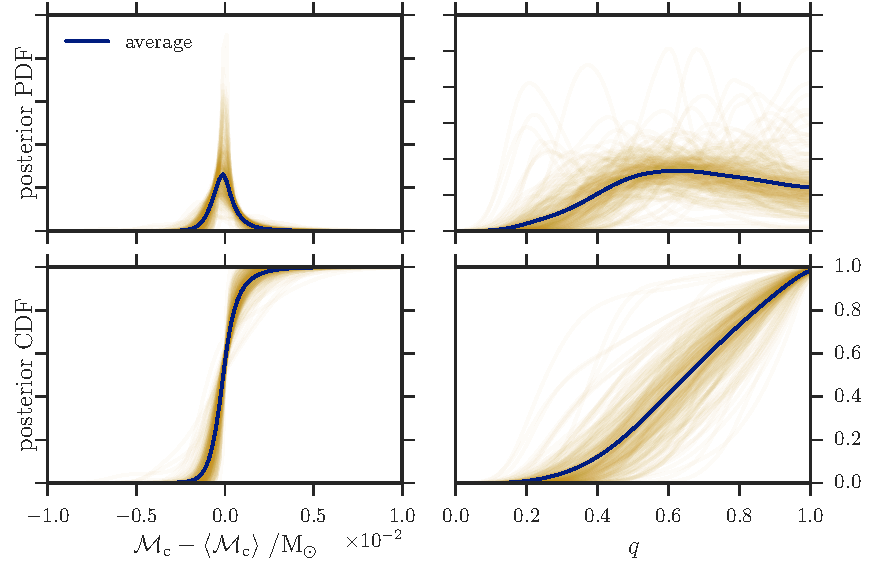
\includegraphics[width=1.6\columnwidth]{mass_pdf_cdfmass_pdf_cdf}
  \caption{\protect\label{fig:mass_pdfs} Superimposed posterior probability density (top) and cumulative density (bottom) functions for the chirp mass and mass ratio of all spinning analyses.  The solid lines show the average distribution for the simulated population.  The chirp-mass distributions have been centered on the distributions' means to highlight their consistent morphology.
  }
\end{figure*}

\begin{figure}
  \centering
  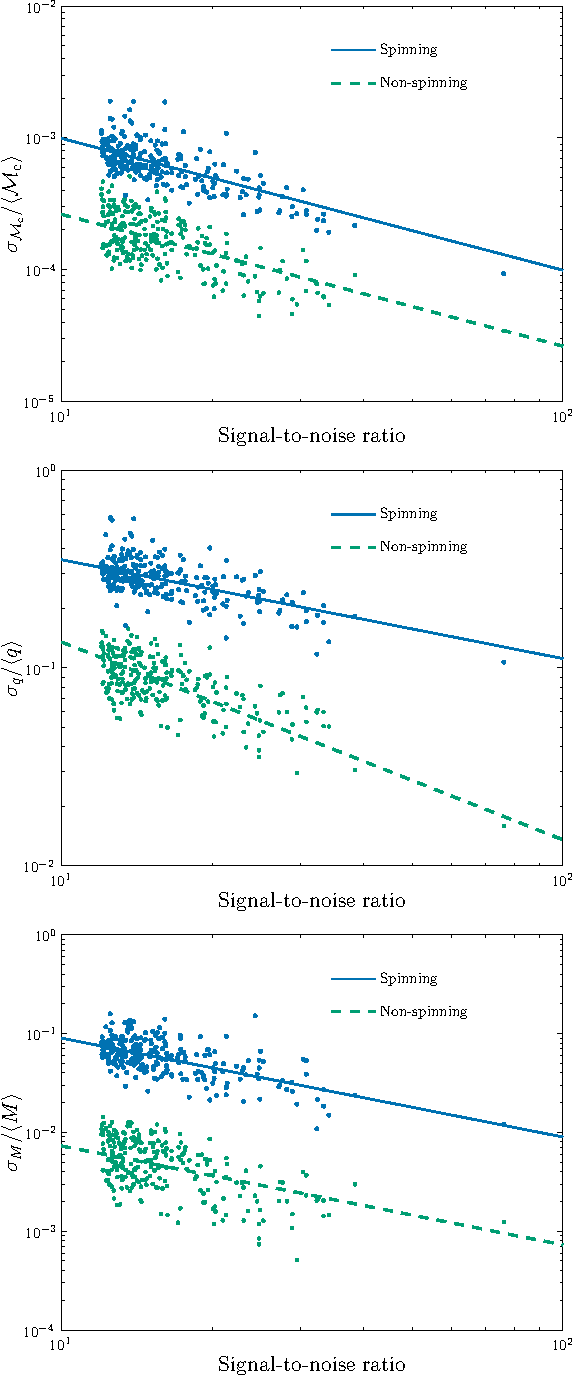
\includegraphics[width=0.85\columnwidth]{mass_snrmass_snr}
  \caption{\protect\label{fig:Mc_q_std_snr} Fractional uncertainties in chirp mass $\mathcal{M}_\mathrm{c}$, mass ratio $q$ and total mass $M$ estimates as a function of network S/N for both the fully spinning SpinTaylorT4 analysis and the medium-latency non-spinning TaylorF2 analysis. We only show statistical uncertainties, not systematic errors (which are present when spin in not included). The lines indicate approximate power-law trends ($\propto \rho_\mathrm{net}^{-1/2}$ for spinning $\sigma_q/\langle q\rangle$ and $\propto \rho_\mathrm{net}^{-1}$ for the rest) to guide the eye.
  
  
  }
\end{figure}

\input{"spin_estimates.tex"}

\begin{figure}
  \centering
  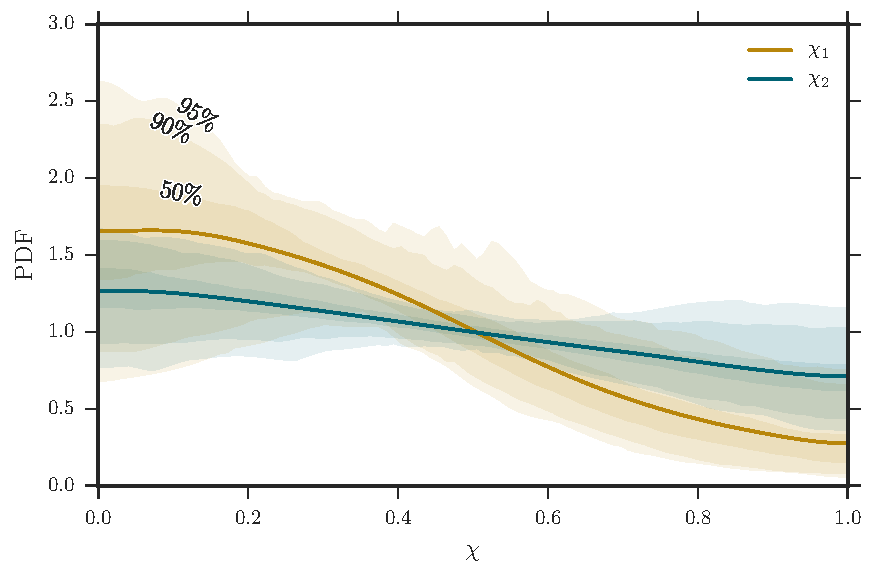
\includegraphics[width=0.95\columnwidth]{spin_cred_regionsspin_cred_regions}
  \caption{\protect\label{fig:spinPDFcred} The distribution of one-dimensional marginalized posterior probability density functions (PDFs) of spin magnitudes of the more and less massive components ($\chi_1$ and $\chi_2$, respectively) for all $250$ simulated sources. Shaded regions show the $90\%$ credible boundaries for the spin distributions of the population, and the solid lines show the average of each PDF.  The posteriors have consistent morphology and span the majority of the prior range.  The spin of the most massive component is typically slightly more constrained toward low values, but even a maximal spin of $\chi_1 = 1$ is never ruled out with $100\%$ certainty.
  
  
  
  }
\end{figure}

\input{"spin_priors.tex"}

\begin{figure}
  \centering
  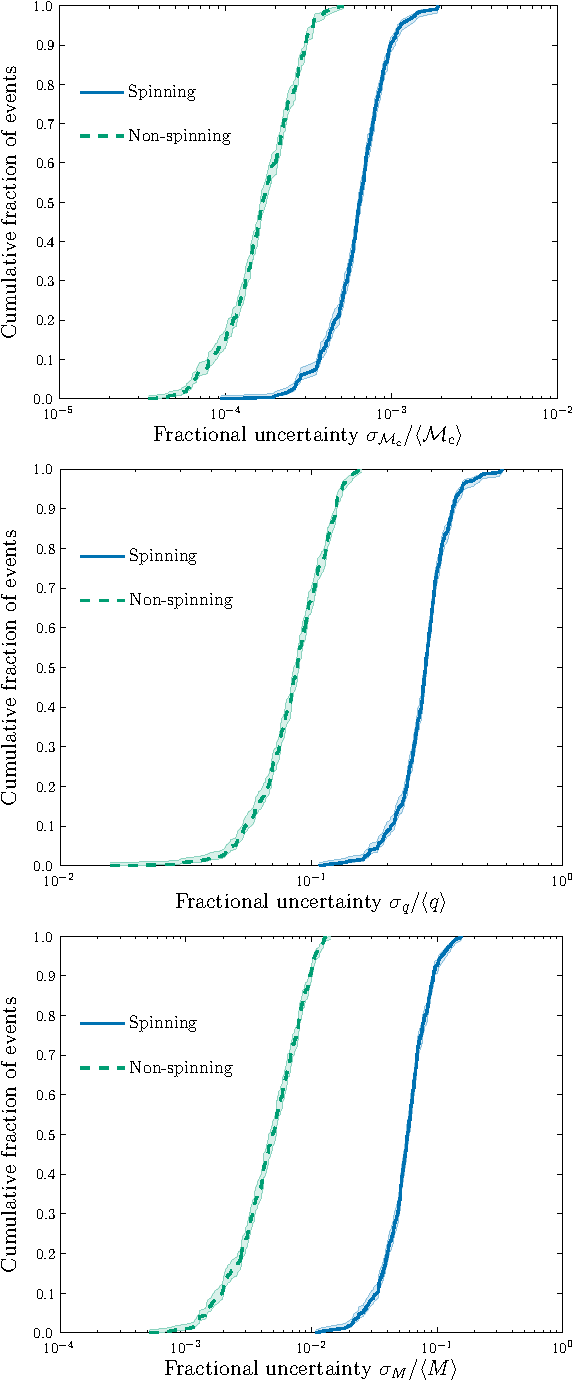
\includegraphics[width=0.85\columnwidth]{mass_fractionalmass_fractional}
  \caption{\protect\label{fig:mass_std} Fractional uncertainty in chirp mass $\mathcal{M}_\mathrm{c}$, mass ratio $q$ and total mass $M$ estimates from the non-spinning and spinning analyses.  The mean fractional uncertainties from the non-spinning analysis are $0.0185\%$, $8.93\%$ and $0.542\%$ for chirp mass, mass ratio and total mass respectively.  These are a factor of a few smaller than found from a spinning analysis ($0.0676\%$, $28.7\%$ and $6.15\%$ for chirp mass, mass ratio and total mass respectively).
  
  
  } 
\end{figure}

\input{"component_masses.tex"}

\begin{figure}
  \centering
  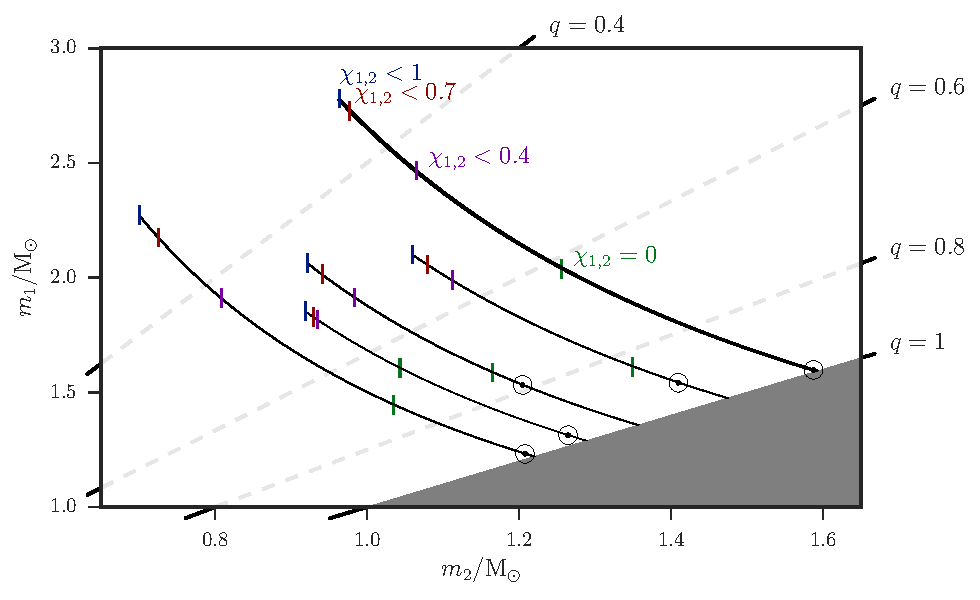
\includegraphics[width=1.0\columnwidth]{mass_compmass_comp}
  \caption{\protect\label{fig:comp_masses} Approximate $90\%$ credible regions for the component-mass estimates of $5$ selected simulations from the spinning analysis; each region is the projection of a rectangular region of chirp-mass--mass-ratio space, bounded by the central $90\%$ credible interval in chirp-mass and upper $90\%$ credible interval in mass-ratio. Circles indicate the true masses of each simulation, and bars indicate the lower bounds of the upper $90\%$ credible intervals (i.e.\ the $10$th percentiles) on mass ratio for increasingly strict prior assumptions on the maximum spin of NSs.}
\end{figure}

\input{"mass_ratio.tex"}

\begin{figure}
  \centering
  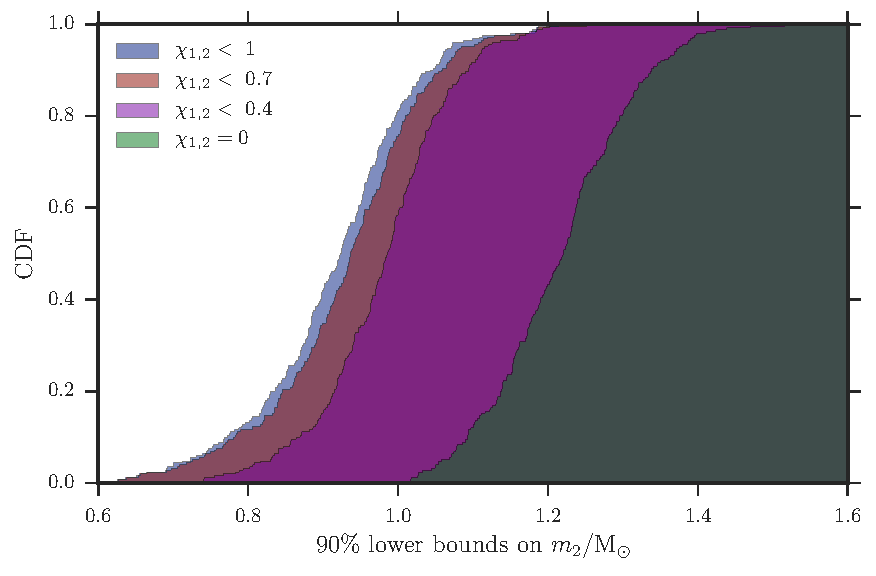
\includegraphics[width=0.95\columnwidth]{mass_secondarymass_secondary}
  \caption{\protect\label{fig:restricted_priors} Cumulative distributions of the lower bounds of the upper $90\%$ credible interval (i.e. $10$th percentiles) on the estimated mass of the least massive binary components under increasingly strict prior assumptions about maximum NS spin.  Restricting spins to be below break-up ($\chi\lesssim0.7$) for non-exotic equations of state has little effect, as does restricting spin to the maximum observed NS spin ($\chi\lesssim0.4$).  Only strict prior assumptions on NS spin will significantly impact mass constraints.
  
  
  
  
  }
\end{figure}

\input{"sky_localization.tex"}

\begin{figure}
  \centering
  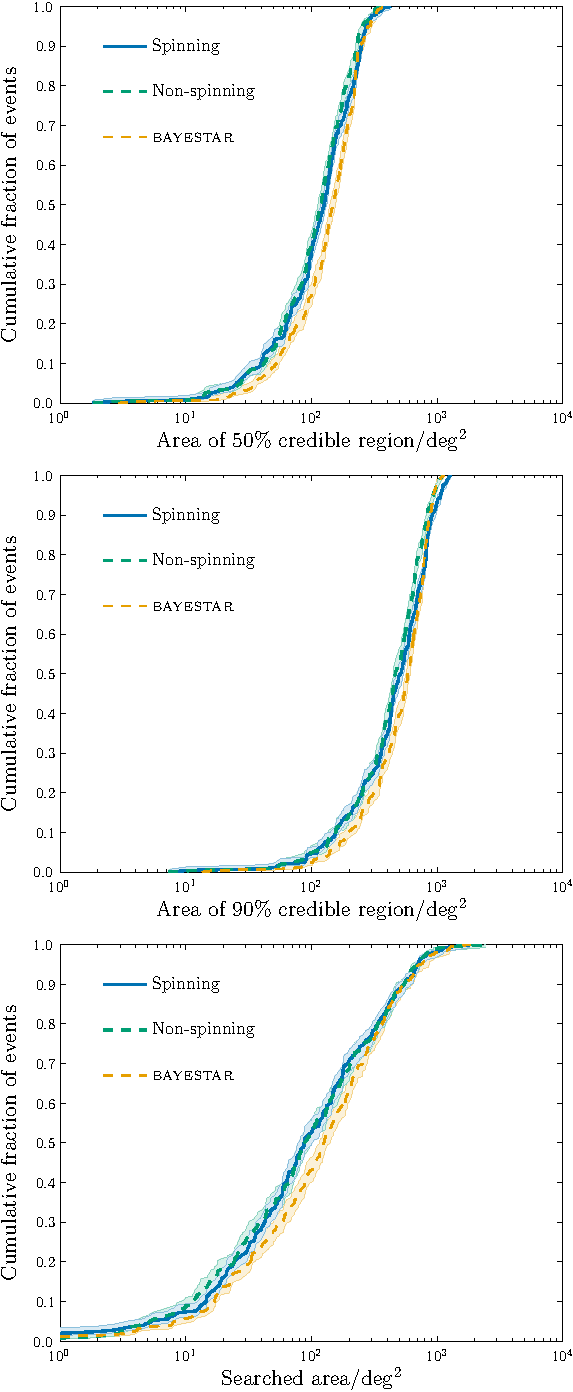
\includegraphics[width=0.85\columnwidth]{sky_areassky_areas}
  \caption{\protect\label{fig:sky} Cumulative fractions of events with sky-localization areas smaller than the abscissa value. Top: Sky area of $50\%$ credible region $\mathrm{CR}_{0.5}$ Middle: Sky area of $\mathrm{CR}_{0.9}$. Bottom: Searched area $A_\ast$. The high-latency results including spin are indicated by the solid (blue) line. The lower latency non-spinning and \textsc{bayestar} from \citet{Singer_2014} are denoted by thicker (green) and thinner (orange) lines respectively. The $68\%$ confidence intervals for the cumulative distribution are denoted by the shaded areas.
  }
\end{figure}

\input{"run-by-run_skyareas.tex"}

\input{"paper-sky-ratio-table.tex"}

\input{"luminosity_distance.tex"}

\begin{figure*}
  \centering
  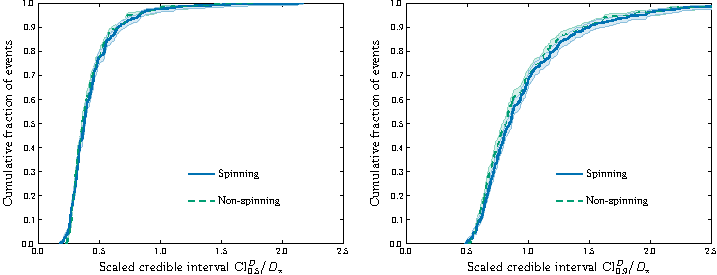
\includegraphics[width=1.7\columnwidth]{spin_distspin_dist}
  \caption{\protect\label{fig:distance} Cumulative fractions of events with luminosity-distance credible intervals (divided by the true distance) smaller than the abscissa value. Left: Scaled $50\%$ credible interval $\mathrm{CI}^{D}_{0.5}/D_\star$. Right: Scaled $90\%$ interval $\mathrm{CI}^{D}_{0.9}/D_\star$. Results using the spinning analysis are indicated by the solid (blue) line and the results using the non-spinning analysis \citep{Berry_2014} are indicated by the dashed (green) line. The $68\%$ confidence intervals for the cumulative distribution are denoted by the shaded areas.
  }
\end{figure*}

\input{"summary.tex"}

\input{"acknowledgements.tex"}

\input{"computational_cost.tex"}

\begin{figure}
  \centering
  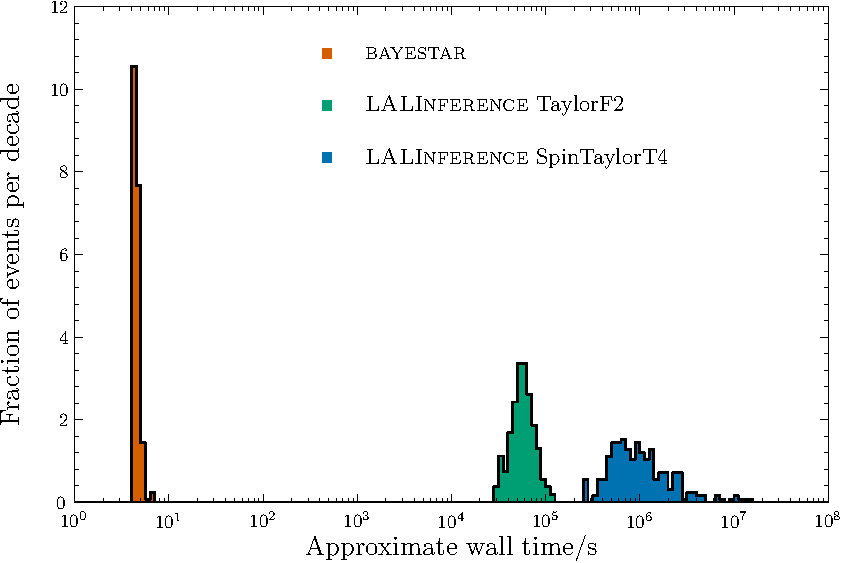
\includegraphics[width=0.95\columnwidth]{time_histtime_hist}
  \caption{\protect\label{fig:wall-time} Distribution of wall times (per event). The left (orange--red) distribution is for low-latency sky localization with \textsc{bayestar}; the middle (green) distribution is for medium-latency non-spinning parameter estimation (performed with \textsc{LALInference\_nest}), and the right (blue) distribution is for low-latency fully spinning parameter estimation (performed with \textsc{LALInference\_MCMC}). The \textsc{bayestar} results assume parallelization across $32$ cores (wall time scales inversely with the number of cores), and both \textsc{LALInference} results assume $2000$ posterior samples (the wall time is approximately proportional to the number of samples).
  
  }
\end{figure}

\bibliographystyle{apj}
\bibliography{bibliography/biblio} 

\end{document}
